% ACL-style Mid-Submission Report — self-contained (no acl.sty needed)
% Compile: pdflatex mid_report  →  bibtex mid_report  →  pdflatex (×2)

\documentclass[11pt,twocolumn]{article}
\usepackage{graphicx}
\usepackage{float}
% ---- Page geometry (matches ACL template) ----
\usepackage[
  paperwidth=210mm, paperheight=297mm,
  top=25mm, bottom=25mm,
  left=17mm, right=17mm,
  columnsep=6mm
]{geometry}

% ---- Fonts & encoding ----
\usepackage[T1]{fontenc}
\usepackage[utf8]{inputenc}
\usepackage{times}
\usepackage{microtype}

% ---- Math ----
\usepackage{amsmath}
\usepackage{amssymb}

% ---- Tables & figures ----
\usepackage{booktabs}
\usepackage{multirow}
\usepackage{graphicx}
\usepackage{array}
\usepackage{xcolor}
\usepackage{tikz}
\usetikzlibrary{positioning,arrows.meta,calc}

% ---- References ----
% natbib with authoryear + round brackets; plainnat.bst is bundled with natbib
\usepackage[round,authoryear]{natbib}

% ---- URLs ----
\usepackage{url}
\usepackage{hyperref}
\hypersetup{colorlinks=true, linkcolor=black, citecolor=black, urlcolor=blue}

% ---- Section style (compact, ACL-like) ----
\usepackage{titlesec}
\titleformat{\section}{\normalfont\large\bfseries}{\thesection}{1em}{}
\titleformat{\subsection}{\normalfont\normalsize\bfseries}{\thesubsection}{1em}{}
\titleformat{\paragraph}[runin]{\normalfont\normalsize\bfseries}{}{0pt}{}[.]
\titlespacing*{\section}{0pt}{8pt}{4pt}
\titlespacing*{\subsection}{0pt}{6pt}{3pt}
\titlespacing*{\paragraph}{0pt}{4pt}{6pt}

% ---- Abstract box ----
\usepackage{abstract}
\setlength{\absleftindent}{0pt}
\setlength{\absrightindent}{0pt}
\renewcommand{\abstractnamefont}{\normalfont\bfseries}

% ---- Caption style ----
\usepackage[font=small,labelfont=bf]{caption}

% ---- Misc layout ----
\setlength{\tabcolsep}{4pt}
\frenchspacing
\setlength{\parindent}{0.25in}
\setlength{\parskip}{0pt}

% --------------------------------------------------------
\title{\Large\bf Multimodal Sentiment Analysis via\\[2pt]
Multi-Layer Feature Fusion and Multi-Task Learning\thanks{Code available at: \url{https://github.com/Gautam-Gandhi/multimodal-sentiment-analysis}}}

\author{
  \textbf{Manas Inamdar} \\ 
  2023102052
  \and
  \textbf{Soham Jahagirdar} \\ 
   2023102046
  \and
  \textbf{Parth Tokekar} \\ 
   2023102041
  \and
  \textbf{Gautam Gandhi} \\ 
   2023102059
}

\date{}

\begin{document}
\maketitle

% ============================================================
\begin{abstract}
Multimodal sentiment analysis (MSA) tries to figure out how positive or negative someone feels by looking at what they say, how they say it, and what their face shows. This report describes where we are in our project of re-implementing the UFEN+MTFN model from \citet{cai2025multimodal}. The model has two parts: UFEN, which learns good features for each modality on its own, and MTFN, which combines all three modalities using cross-modal attention and a Transformer encoder-decoder. We trained our model on the CMU-MOSI dataset and currently achieve a binary accuracy (neg/pos) of 77.7\% and Pearson correlation of 0.618 with 442K parameters. We explain what we built, what results we have, why our numbers are below the paper's target, and what we plan to do next to close that gap.
\end{abstract}

% ============================================================
\section{Introduction}
\label{sec:intro}

When people talk, they send information through several channels at the same time. Their words carry meaning. Their voice carries emotion through tone and pace. Their face shows reactions through expressions. Multimodal Sentiment Analysis (MSA) is the task of automatically deciding whether a person is being positive or negative by looking at all these channels together, rather than reading the words alone.

This matters in many real situations. Think of a customer review video online. The person might say ``it was fine'' but their voice sounds flat and their face looks disappointed. A system that only reads the words will miss the real feeling. By combining text, audio, and video, we can build systems that understand people much more accurately.

\subsection{Why Is This Problem Hard?}

Making three very different types of data work together is not simple. There are three main problems.

\textbf{The data looks completely different across modalities.} Text is a sequence of 768-number word embeddings from BERT. Audio is a sequence of 74 acoustic measurements per time step. Video is a sequence of 35 face movement measurements per time step. These numbers live in totally different spaces and cannot be compared directly. A model needs to first put them all into a common space before they can be combined.

\textbf{The modalities often say opposite things.} This is especially common with sarcasm. Someone might say ``I absolutely loved it'' while their voice is flat and their face is blank or even frowning. If we just average the signals from each modality, the conflicting ones cancel each other out and we get the wrong answer. A good model needs to decide which modality to trust more in each case.

\textbf{Text is much more useful than audio or video for sentiment.} In the CMU-MOSI dataset, if you only use text features you already get around 73\% accuracy. Audio and video add only a few extra points. But those few points matter, and the cases where audio and video help are often exactly the hard cases (like sarcasm). So a model cannot just ignore audio and video even though they are weaker signals.

\subsection{Our Approach}

The paper we are re-implementing, \citet{cai2025multimodal}, handles all three problems with a two-stage design. In Stage 1, a network called UFEN processes each modality by itself. It uses a combination of recurrent layers, convolution, and self-attention to build a good, compact representation for each modality independently. In Stage 2, a network called MTFN takes these three representations and applies cross-modal attention across all six possible directed pairs. This lets each modality ``look into'' the others to find information it is missing. Finally, a Transformer encoder-decoder block refines the combined result.

The training also uses five separate losses, one for each of the three modalities alone and two for the combined result. This forces the model to keep all three modalities useful throughout training, rather than learning to ignore the weaker ones.

\subsection{Our Contributions}

We are implementing this model from scratch in PyTorch. The specific things we have done so far are:

\begin{itemize}
    \item A full PyTorch implementation of both UFEN and MTFN, with every design choice documented, including the parts the original paper did not fully describe.
    \item A complete training and evaluation pipeline for CMU-MOSI, including proper data loading, Z-score normalisation with training-set statistics, gradient clipping, early stopping, and all five standard metrics.
    \item A working model with 442,501 parameters that achieves Acc-2 (neg/pos) = 77.7\% and Pearson correlation = 0.618, giving us a solid starting baseline.
    \item An ablation study confirming which parts of the model matter most, plus a clear explanation of why our numbers are lower than the paper's target.
\end{itemize}

% ============================================================
\section{Related Work}
\label{sec:related}

\subsection{Representing Each Modality}

Early MSA systems used hand-designed features. For text, people counted words or used n-gram vectors. For audio, they measured average pitch or energy. For video, they tracked which facial muscles were moving. These features were easy to build but not very powerful.

Deep learning made a big difference. LSTM and GRU networks could read a sequence of features and learn what patterns meant positive or negative sentiment \citep{poria2017review}. The biggest jump in text quality came from BERT \citep{devlin2019bert}, which reads an entire sentence and gives each word a vector that depends on its context. For example, the word ``sick'' has a completely different meaning in ``that performance was sick'' (slang for great) versus ``I felt sick'' (ill). BERT handles this naturally. COVAREP \citep{degottex2014covarep} provides a standard set of voice quality measurements for audio, and FACET 4.2 provides facial action unit measurements for video. These three feature extractors together are now the standard starting point for CMU-MOSI experiments.

\subsection{Combining Modalities (Fusion)}

There are three general families of fusion strategies: early, late, and attention-based fusion.

\textbf{Early fusion} combines features before training. The simplest version concatenates all feature vectors into one big vector and feeds it into a neural network \citep{zadeh2016multimodal}. This is fast but ignores the fact that text, audio, and video have very different structures.

\textbf{Tensor Fusion (TFN)} \citep{zadeh2017tensor} takes early fusion further. It computes the outer product of all three modality vectors, which creates a tensor that explicitly represents every combination of features from all three modalities at once. The problem is that this tensor is huge: if each modality vector has $d$ dimensions, the tensor has $d^3$ elements. Low-rank Multimodal Fusion (LMF) \citep{liu2018efficient} fixes this by factorising the weight tensors into smaller pieces, which gives similar accuracy at much lower computation cost.

\textbf{Late fusion} trains a separate model for each modality and combines their predictions at the end. This is simple but cannot model interactions between modalities at the feature level.

\textbf{Attention-based fusion} is the most powerful modern approach. The key idea is that instead of just stacking or averaging features, we let each modality gather relevant information from the others using attention. The Multimodal Transformer (MulT) \citep{tsai2019multimodal} applies cross-modal attention so the text can attend to audio time steps and vice versa. This works well even when the modalities are not aligned in time. Memory Fusion Network (MFN) \citep{zadeh2018memory} stores multi-view interactions in an explicit memory and updates it at every step. Graph-MFN \citep{zadeh2018multimodal} extends this into a graph structure. MISA \citep{hazarika2021misa} separates each modality's representation into two parts: one that captures what all modalities share, and one that captures what is unique to that modality.

\subsection{Multi-Task Learning for Sentiment}

A common problem in MSA training is that the model learns to mostly rely on text, since text is so much more informative than audio or video. Multi-task learning is a way to fight this.

The idea is to make the model predict the sentiment score not just from the combined features, but also from each modality alone. This forces the model to make each modality representation useful by itself, which in turn makes the combined result better.

Self-MM \citep{yu2021selfmm} is a strong example of this approach. It automatically generates separate sentiment labels for each modality using a self-supervised algorithm, then uses these as targets for per-modality heads. This achieves much better results than training with only one combined output. MMIM \citep{han2021improving} is similar in spirit but uses information-theoretic objectives: it maximises the mutual information between each modality's features and the final prediction.

The model we are re-implementing \citep{cai2025multimodal} combines cross-modal attention fusion with multi-task learning. It builds on the ideas of both MulT and Self-MM, and adds a Transformer encoder-decoder on top for an extra refinement step. Our job is to re-implement and understand all of these pieces.

% ============================================================
\section{Dataset}
\label{sec:dataset}

\subsection{CMU-MOSI Overview}

We use the \textbf{CMU-MOSI} dataset \citep{zadeh2016multimodal} for all experiments. CMU-MOSI contains 2,199 short video clips taken from YouTube movie review videos. Each clip is one sentence (called an utterance). A human gave each clip a sentiment score between $-3$ (very negative) and $+3$ (very positive). A score of $+1$ or $+2$ is mildly positive, $-1$ or $-2$ is mildly negative, $+3$ or $-3$ are at the extremes.

CMU-MOSI is the most common benchmark for MSA. Almost every paper in this area reports results on it, which makes it easy to compare methods. It does come with some challenges though. The dataset is small (only 1,283 training samples), which means models can easily overfit. The label distribution is also slightly unbalanced, with more negative samples than positive ones. These properties make it a good but difficult testbed.

\subsection{Modality Features}

We use the standard pre-extracted, word-aligned features. We do not extract features ourselves. The three modality feature sets are described below.

\textbf{Text ($d_t = 768$).} Each word in the sentence is a 768-dimensional vector from BERT-base-uncased \citep{devlin2019bert}. BERT reads the full sentence simultaneously and gives each word a representation that reflects its meaning given all the other words around it. We use BERT as a fixed feature extractor at this stage (no fine-tuning).

\textbf{Audio ($d_a = 74$).} Each time step of the audio is described by 74 numbers from the COVAREP toolkit \citep{degottex2014covarep}. These 74 numbers measure voice properties like pitch (how high or low the voice is), formants (the resonance of the vocal tract), and glottal source parameters (properties of how the vocal cords vibrate). Together they give a compact description of the speaker's voice quality at each moment.

\textbf{Visual ($d_v = 35$).} Each video frame is described by 35 numbers from the FACET 4.2 toolkit. These cover facial action units (which face muscles are active), eye openness, and geometric measurements like the distance between the eyes. The visual features are the weakest predictor of sentiment on their own but can help in cases where the face clearly contradicts the words.

\subsection{Preprocessing Steps}

All sequences are padded or cut to exactly $T = 30$ time steps. This gives every sample the same shape, which is required for batched training.

The audio and visual features have a known quality problem: some frames contain extremely large negative values (around $-3.4 \times 10^{38}$) because COVAREP fills silent frames with these placeholder values. If we do not remove them, the Z-score normalisation step will produce useless statistics. Our preprocessing pipeline handles this in order:

\begin{enumerate}
    \item Clip all values to the range $[-10^4, 10^4]$ to remove the extreme placeholders.
    \item Replace any remaining NaN or infinity values with zero.
    \item Compute mean and standard deviation from the training set only, then apply these to all three splits (train, val, test).
\end{enumerate}

We do not normalise the BERT text features. BERT produces values in a reasonable range already, and changing them could harm the representations.

\subsection{Data Splits}

The train/val/test splits are fixed for CMU-MOSI and are the same across all published papers (Table~\ref{tab:dataset}).

\begin{table}[h]
\centering
\small
\begin{tabular}{lccc}
\toprule
\textbf{Split} & \textbf{Samples} & \textbf{Label range} & \textbf{Modalities} \\
\midrule
Train      & 1,283 & $[-3, +3]$ & Text / Audio / Visual \\
Validation & 214   & $[-3, +3]$ & Text / Audio / Visual \\
Test       & 686   & $[-3, +3]$ & Text / Audio / Visual \\
\bottomrule
\end{tabular}
\caption{CMU-MOSI dataset splits. All modalities are available for every sample.}
\label{tab:dataset}
\end{table}

% ============================================================
\section{Methodology}
\label{sec:method}

\subsection{Task Definition}

The input is one video clip described by three sequences: text $X_t \in \mathbb{R}^{T \times 768}$, audio $X_a \in \mathbb{R}^{T \times 74}$, and visual $X_v \in \mathbb{R}^{T \times 35}$, all padded to $T = 30$ steps. The output is a single number predicting sentiment on the $[-3, +3]$ scale.

During training the model produces five outputs: three unimodal predictions ($Y_t$, $Y_a$, $Y_v$), a combined prediction from the cross-modal attention block ($Y_m$), and a final refined prediction from the encoder-decoder ($Y_{m'}$). At test time only $Y_{m'}$ is used.

\subsection{Overall Architecture}

The pipeline has two stages, shown in Figure~\ref{fig:arch}.

\begin{figure}[t]
\centering
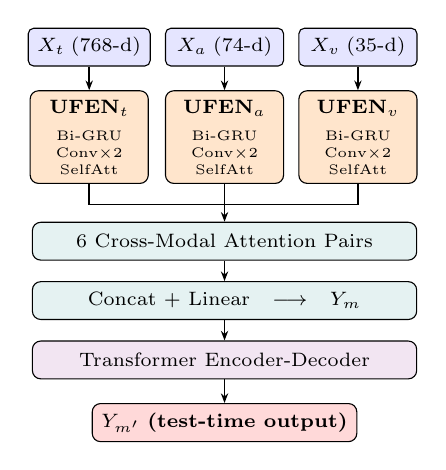
\begin{tikzpicture}[
  node distance=0.3cm and 0.18cm,
  inp/.style={draw, rounded corners=2pt, fill=blue!10,
              minimum width=1.5cm, minimum height=0.48cm,
              align=center, font=\scriptsize},
  ufen/.style={draw, rounded corners=3pt, fill=orange!20,
               minimum width=1.5cm, minimum height=1.05cm,
               align=center, font=\scriptsize},
  wide/.style={draw, rounded corners=3pt, fill=teal!10,
               minimum width=4.88cm, minimum height=0.48cm,
               align=center, font=\scriptsize},
  mfuse/.style={draw, rounded corners=3pt, fill=violet!10,
                minimum width=4.88cm, minimum height=0.48cm,
                align=center, font=\scriptsize},
  finaln/.style={draw, rounded corners=3pt, fill=red!15,
                 minimum width=2.6cm, minimum height=0.48cm,
                 align=center, font=\scriptsize\bfseries},
  arr/.style={-{Stealth[length=3.5pt]}, semithick},
  line/.style={semithick},
]

%% Inputs
\node[inp] (xt) {$X_t$\;(768-d)};
\node[inp, right=0.18cm of xt] (xa) {$X_a$\;(74-d)};
\node[inp, right=0.18cm of xa] (xv) {$X_v$\;(35-d)};

%% UFEN blocks
\node[ufen, below=0.3cm of xt] (ut)
  {\textbf{UFEN}$_t$\\[2pt]{\tiny Bi-GRU}\\[-2pt]{\tiny Conv$\times$2}\\[-2pt]{\tiny SelfAtt}};
\node[ufen, below=0.3cm of xa] (ua)
  {\textbf{UFEN}$_a$\\[2pt]{\tiny Bi-GRU}\\[-2pt]{\tiny Conv$\times$2}\\[-2pt]{\tiny SelfAtt}};
\node[ufen, below=0.3cm of xv] (uv)
  {\textbf{UFEN}$_v$\\[2pt]{\tiny Bi-GRU}\\[-2pt]{\tiny Conv$\times$2}\\[-2pt]{\tiny SelfAtt}};

\draw[arr](xt)--(ut);
\draw[arr](xa)--(ua);
\draw[arr](xv)--(uv);

%% Funnel merge point
\coordinate (merge) at ($(ua.south)+(0,-0.26)$);
\draw[line](ut.south) |- (merge);
\draw[line](ua.south)  -- (merge);
\draw[line](uv.south) |- (merge);

%% Cross-modal attention
\node[wide, below=0.48cm of ua] (ca)
  {6 Cross-Modal Attention Pairs};
\draw[arr](merge)--(ca);

%% Concat + Ym
\node[wide, below=0.26cm of ca] (concat)
  {Concat $+$ Linear\quad$\longrightarrow$\quad$Y_m$};
\draw[arr](ca)--(concat);

%% Encoder-Decoder
\node[mfuse, below=0.26cm of concat] (ed)
  {Transformer Encoder-Decoder};
\draw[arr](concat)--(ed);

%% Final output
\node[finaln, below=0.3cm of ed] (ym)
  {$Y_{m'}$\;(test-time output)};
\draw[arr](ed)--(ym);

\end{tikzpicture}
\caption{The UFEN+MTFN architecture. Each UFEN independently processes one modality (Bi-GRU, Conv$\times$2, SelfAtt) and also produces a unimodal prediction ($Y_t, Y_a, Y_v$) used only during training. MTFN fuses all three representations via six directed cross-modal attention pairs, then refines the result through a Transformer encoder-decoder to give $Y_{m'}$, the final test-time output.}
\label{fig:arch}
\end{figure}

\textbf{Stage 1 (UFEN)} runs the same multi-step feature extraction pipeline on each modality separately. Three independent UFEN networks (one per modality) each output a feature sequence of shape $T \times d_m$.

\textbf{Stage 2 (MTFN)} takes these three sequences and combines them using six directed cross-modal attention operations. The results are concatenated, projected to a first prediction $Y_m$, then passed through a Transformer encoder-decoder to get the final prediction $Y_{m'}$.

\begin{figure}[H]
    \centering
    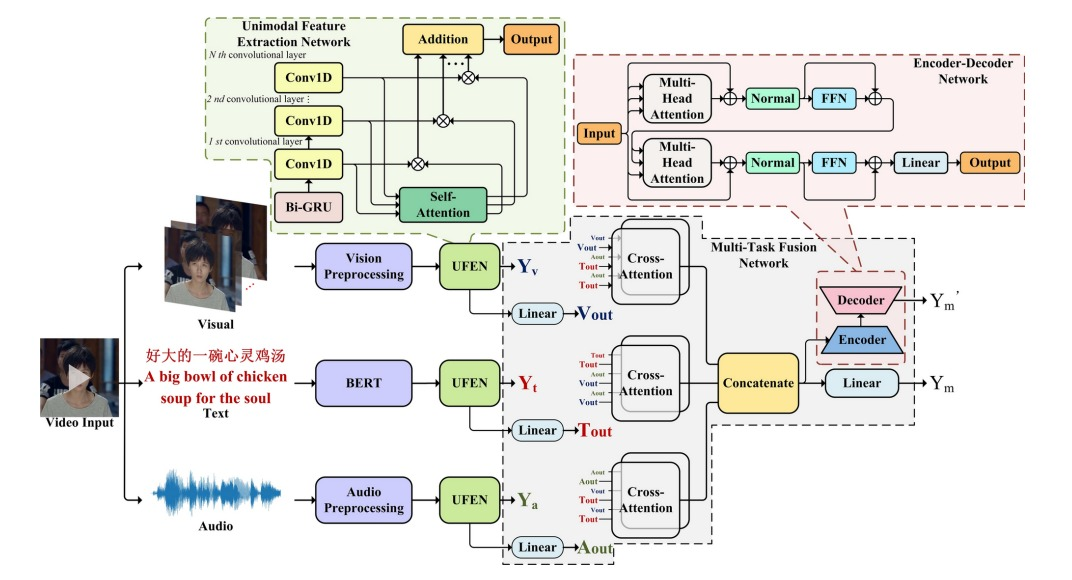
\includegraphics[width=1\linewidth]{arch.png}
    \caption{The overall architecture of our method. The Ym, Yt, Ya, Yv, Ym'
 are the prediction outputs of the multi-modal task, the three single-modal tasks and the fusion feature reconstruction task respectively. Ym' is used as the multimodal sentiment output.}
    \label{fig:placeholder}
\end{figure}

\subsection{Stage 1: UFEN in Detail}
\label{sec:ufen}

UFEN has five steps. All three modality networks share the same structure but have their own separate weights.

\paragraph{Step 1 -- Bi-GRU.}
The raw input $X_i \in \mathbb{R}^{T \times D_i}$ is read by a bidirectional GRU:
\begin{equation}
X_i^{\text{BiGRU}} = \text{BiGRU}(X_i) \in \mathbb{R}^{T \times d_m}
\end{equation}
where $d_m = 2h$, $h = 32$ per direction so $d_m = 64$. Reading the sequence in both directions helps because sentiment often depends on context that comes later. For example, ``not bad at all'' is positive, but if we only read left to right the word ``bad'' might be misleading.

\paragraph{Step 2 -- Two Conv1D layers.}
We apply $l = 2$ stacked 1D convolutional layers:
\begin{equation}
X_i^{\text{layer}} = \text{Conv1D}^{\text{layer}}\!\left(X_i^{\text{BiGRU}},\; K{=}3,\; F{=}64\right)
\end{equation}
Each convolution looks at 3 consecutive time steps at once and learns what local patterns are important. The first layer detects simple local features; the second builds on these to detect slightly wider patterns. Same-padding keeps the output length at $T$.

\paragraph{Step 3 -- Self-Attention Gate.}
After each convolution, we apply a self-attention mechanism:
\begin{equation}
\text{Attention}(X) = \text{softmax}\!\left(\frac{X X^T}{\sqrt{d_k}}\right) X
\end{equation}
This lets each time step look at all other time steps and decide how much attention to give them. The output is used as a multiplicative gate on the convolution output:
\begin{align}
X_i^{\text{layerAtt}} &= \text{Attention}(X_i^{\text{layer}}) \\
X_i^{\text{self-att}} &= X_i^{\text{layer}} \otimes X_i^{\text{layerAtt}}
\end{align}
where $\otimes$ is element-wise multiplication. Time steps that are more important for sentiment get amplified; less relevant ones get scaled down. This is different from regular self-attention because the output is used as a \emph{gate}, not added back.

\paragraph{Step 4 -- Sum across layers.}
Each gated output is projected back to size $d_m$ and all layers are added:
\begin{align}
X_{\text{layer}} &= \text{Linear}(X_i^{\text{self-att}}) \in \mathbb{R}^{T \times d_m} \\
X_i^{\text{fusion}} &= X_1 \oplus X_2 \oplus \cdots \oplus X_l
\end{align}
where $\oplus$ is element-wise addition. Adding layer outputs (instead of using only the last one) means the final representation keeps both the local patterns from layer 1 and the broader patterns from layer 2.

\paragraph{Step 5 -- Unimodal prediction head.}
We average across time and apply a linear layer:
\begin{equation}
Y_i = W_i \cdot \text{MeanPool}(X_i^{\text{fusion}}) + b_i
\end{equation}
This prediction is used only during training as part of the multi-task loss. It forces each UFEN to learn a meaningful representation that can predict sentiment on its own.

\subsection{Stage 2: MTFN in Detail}
\label{sec:mtfn}

\paragraph{Cross-modal attention.}
The central idea of MTFN is that each modality can help fill in gaps in the others. The audio signal might confirm that a sentence is sarcastic; the visual signal might confirm that a neutral-sounding sentence is actually angry. Cross-modal attention allows modality $i$ to query the other modality $j$ and pull out the information it needs.

For each ordered pair $(i, j)$, we project both sequences to a shared dimension $D_e = 64$ and compute multi-head attention with modality $i$ as the query and modality $j$ as key/value:
\begin{align}
Q_i &= W_{Q_i} W_i X_i, \quad K_j = W_{K_j} W_j X_j \nonumber\\
V_j &= W_{V_j} W_j X_j \\
\text{CA}_{i \to j} &= \text{LN}\!\left(\text{MHAtt}(Q_i, K_j, V_j)\right)
\end{align}
The projection matrices $W_i$ per modality are shared across all pairs involving that modality. This means text always maps to the same embedding space regardless of whether it is acting as query or being queried. All six directed pairs are computed: text$\to$audio, text$\to$visual, audio$\to$text, audio$\to$visual, visual$\to$text, visual$\to$audio. Each gives a tensor of shape $(B, T, D_e)$.

\paragraph{Concatenation and first multimodal prediction.}
The six attention outputs are averaged over the time dimension and joined together:
\begin{equation}
\text{Fused} = \text{Concat}\!\left[\text{MeanPool}(\text{CA}_{i \to j})\right]_{(i,j)} \in \mathbb{R}^{6 D_e}
\end{equation}
A linear layer maps this to the first multimodal prediction:
\begin{equation}
Y_m = W_m \cdot \text{Fused} + b_m
\end{equation}

\paragraph{Transformer encoder-decoder.}
The fused vector has 6 chunks of size $D_e$, so we reshape it to $(B, 6, D_e)$ and treat it as a 6-element sequence. One Transformer encoder block refines this sequence:
\begin{align}
Z_{\text{enc}} &= \text{LN}\bigl(\text{Input} + \text{MHAtt}(\text{Input})\bigr) \\
\text{Out}_{\text{enc}} &= \text{LN}\bigl(Z_{\text{enc}} + \text{FFN}(Z_{\text{enc}})\bigr)
\end{align}
One Transformer decoder block then uses $\text{Out}_{\text{enc}}$ as context:
\begin{align}
Z_{\text{dec}} &= \text{LN}\bigl(\text{Input} + \text{MHAtt}(\text{Input},\,\text{Out}_{\text{enc}})\bigr) \\
\text{Out}_{\text{dec}} &= \text{LN}\bigl(Z_{\text{dec}} + \text{FFN}(Z_{\text{dec}})\bigr)
\end{align}
Averaging over the 6 positions and projecting gives the final prediction:
\begin{equation}
Y_{m'} = W_{de}\cdot\text{MeanPool}(\text{Out}_{\text{dec}}) + b_{de}
\end{equation}
$Y_{m'}$ is the output used at test time.

\subsection{Multi-Task Loss}

All five predictions are trained simultaneously. The total loss is the sum of five MSE losses:
\begin{equation}
\mathcal{L}_{\text{total}} = \mathcal{L}_t + \mathcal{L}_a + \mathcal{L}_v + \mathcal{L}_f + \mathcal{L}_{\text{ed}}
\end{equation}
where each term is:
\begin{equation}
\mathcal{L}_x = \frac{1}{N} \sum_{n=1}^{N} (Y^n - \hat{Y}_x^n)^2
\end{equation}
All five use the same ground-truth label. The three unimodal losses are the key to making multi-task learning work. Without them the model can ignore audio and visual completely, since text alone already gives a decent accuracy. The unimodal losses prevent this by directly penalising poor unimodal predictions.

\subsection{Design Decisions}

The original paper leaves several hyperparameters unspecified. Table~\ref{tab:hparam} shows every setting we use, labelled as either coming from the paper or chosen by us. The most important missing values are the GRU hidden size, the encoder-decoder hidden size, and the conv filter size. We chose $d_m = D_e = F = 64$ as a reasonable starting point for a small dataset.

\begin{table}[t]
\centering
\small
\begin{tabular}{lll}
\toprule
\textbf{Hyperparameter} & \textbf{Value} & \textbf{Source} \\
\midrule
Learning rate & $5 \times 10^{-3}$ & Paper (Table 2) \\
Batch size & 32 & Paper (Table 2) \\
Max epochs & 30 & Paper (Table 2) \\
Early stop patience & 8 & Paper (Table 2) \\
Optimizer & Adam & Paper \\
Loss function & MSE & Paper \\
Self-Att heads & 1 & Paper (Table 2) \\
Cross-Att heads & 4 & Paper (Table 2) \\
Att dropout & 0.2 & Paper (Table 2) \\
Dropout & 0.1 & Paper (Table 2) \\
Conv layers ($l$) & 2 & Paper (ablation) \\
\midrule
$d_m$ (GRU hidden $\times 2$) & 64 & Assumed \\
$D_e$ (cross-att dim) & 64 & Assumed ($= d_m$) \\
Conv kernel size $K$ & 3 & Assumed \\
Conv filters $F$ & 64 & Assumed ($= d_m$) \\
Enc/Dec heads & 4 & Assumed \\
FFN dim & 256 & Assumed ($4 \times d_m$) \\
\midrule
Trainable parameters & 442,501 & Measured \\
\bottomrule
\end{tabular}
\caption{All hyperparameters used. ``Assumed'' values are not given in the paper.}
\label{tab:hparam}
\end{table}

% ============================================================
\section{Experimental Setup}
\label{sec:experiments}

\subsection{Implementation}

We wrote the full model in PyTorch 2.0. All experiments run on an NVIDIA RTX 3050 Laptop GPU. Each training run finishes in about 5--8 minutes. We split the code into separate files for dataset loading (\texttt{dataset.py}), each model component (\texttt{ufen.py}, \texttt{mtfn.py}, \texttt{msa\_model.py}), metrics (\texttt{metrics.py}), and training (\texttt{train.py}). A JSON config file controls all hyperparameters so we can run experiments without changing any code.

We use the Adam optimizer with learning rate $5 \times 10^{-3}$. We also tried applying gradient clipping at norm 1.0. The paper does not mention this, but without it the training occasionally diverges in the first few epochs due to very large gradient values. Clipping fixed this completely.

\subsection{Evaluation Metrics}

We compute six metrics on the test set, following the CMU-MOSI standard protocol \citep{yu2021selfmm, hazarika2021misa}:

\begin{itemize}
    \item \textbf{Acc-2 (nn/np)}: Binary accuracy deciding positive vs.\ negative. ``nn'' uses all samples with threshold 0. ``np'' uses only non-zero labelled samples, threshold 0. The ``np'' version is the main metric most papers report.
    \item \textbf{F1 (nn/np)}: F1-score for the same two binary classifications.
    \item \textbf{MAE}: Mean absolute error on the continuous $[-3,+3]$ scale. Lower is better.
    \item \textbf{Corr}: Pearson correlation between our predictions and the true labels.
    \item \textbf{Acc-7}: Accuracy when both predictions and labels are rounded to the nearest integer (7 possible values from $-3$ to $+3$).
\end{itemize}

Higher is better for all metrics except MAE.

\subsection{Baselines}

We compare against results from the original paper for: \textbf{EF-LSTM} \citep{zadeh2016multimodal}, \textbf{LF-DNN}, \textbf{TFN} \citep{zadeh2017tensor}, \textbf{LMF} \citep{liu2018efficient}, \textbf{MFN} \citep{zadeh2018memory}, \textbf{Graph-MFN} \citep{zadeh2018multimodal}, \textbf{MulT} \citep{tsai2019multimodal}, \textbf{MISA} \citep{hazarika2021misa}, \textbf{Self-MM} \citep{yu2021selfmm}, and \textbf{MMIM} \citep{han2021improving}.

\subsection{Implementation Challenges}

During this project we ran into several problems that the paper did not describe.

\textbf{Bad audio/visual values.} The COVAREP features had extreme values (around $-3.4 \times 10^{38}$) in silent frames. These made the Z-score normalisation completely fail since the mean and standard deviation became meaningless. We fixed this by clipping to $[-10^4, 10^4]$ and zeroing NaN/inf values before computing normalisation statistics.

\textbf{Gradient explosion.} In the first few training epochs, gradient values grew very large and caused the loss to jump or become NaN. Adding gradient clipping (max norm = 1.0) solved this immediately. We think the original authors may have used a learning rate warmup period instead, but they do not document it.

\textbf{Missing hyperparameters.} As shown in Table~\ref{tab:hparam}, the paper leaves several key dimensions unspecified. Our assumed values give us 442K parameters and reasonable accuracy, but the actual values could be much larger.

\textbf{Padding masks.} All three modalities are padded to $T = 30$. If the padding tokens are included in attention computations, attention scores are wasted on meaningless zero-padded positions. We verified with unit tests that padding masks are passed correctly to all attention layers.

% ============================================================
\section{Results and Analysis}
\label{sec:results}

\subsection{Main Results on CMU-MOSI}

Table~\ref{tab:mosi_results} compares our model to all baselines and the paper's target.

\begin{table*}[t]
\centering
\small
\begin{tabular}{lccccc}
\toprule
\textbf{Model} & \textbf{Acc-2 (nn/np)} & \textbf{F1 (nn/np)} & \textbf{MAE$\downarrow$} & \textbf{Corr} & \textbf{Acc-7} \\
\midrule
EF-LSTM         & 77.8 / 79.0 & 77.7 / 78.9 & 0.952 & 0.651 & 34.5 \\
LF-DNN          & 78.0 / 79.3 & 77.9 / 79.3 & 0.978 & 0.658 & 33.6 \\
TFN             & --- / 80.8  & --- / 80.7  & 0.901 & 0.698 & 32.1 \\
LMF             & --- / 82.5  & --- / 82.4  & 0.917 & 0.695 & 32.8 \\
MFN             & 77.4 / ---  & 77.3 / ---  & 0.965 & 0.632 & 34.1 \\
Graph-MFN       & 77.9 / 80.2 & 77.8 / 80.1 & 0.939 & 0.656 & 34.4 \\
MulT            & 81.5 / 84.1 & 80.6 / 83.9 & 0.861 & 0.711 & 40.0 \\
MISA            & 81.8 / 83.4 & 81.7 / 83.6 & 0.783 & 0.761 & 42.3 \\
Self-MM         & 82.5 / 83.8 & 82.5 / 83.9 & 0.758 & 0.779 & 44.9 \\
MMIM            & 80.2 / 81.9 & 80.2 / 82.0 & 0.811 & 0.725 & 45.0 \\
\midrule
\citet{cai2025multimodal} (target) & \textbf{85.2 / 86.6} & \textbf{85.2 / 86.7} & \textbf{0.728} & \textbf{0.792} & \textbf{46.7} \\
\midrule
\textbf{Ours (current)} & 75.5 / 77.7 & 75.1 / 77.5 & 0.981 & 0.618 & 34.3 \\
\bottomrule
\end{tabular}
\caption{Results on the CMU-MOSI test set. Lower MAE is better; all other metrics higher is better. ``nn'' = all samples; ``np'' = non-zero samples. Baseline numbers are from \citet{cai2025multimodal}.}
\label{tab:mosi_results}
\end{table*}

Our model gets \textbf{Acc-2 (np) = 77.7\%} and \textbf{Corr = 0.618}. This puts us roughly at the same level as EF-LSTM and Graph-MFN, both of which are much simpler models. There is a gap of about 9 percentage points between us and the paper's reported best of 86.6\%.

\subsection{Why Is There a Gap?}

\paragraph{The hidden size is probably too small.} The original paper does not say what size the GRU hidden state or the attention dimensions should be. We chose $d_m = 64$, giving 442K parameters. If the authors used $d_m = 128$ the model would have about 1.5 million parameters, and at $d_m = 256$ about 5 million. Larger models can fit the training data better. This is likely the single biggest cause of the accuracy gap, and it is the first thing we will test next.

\paragraph{We do not fine-tune BERT.} We use BERT as a fixed feature extractor. The paper says they use BERT but does not clearly state whether they fine-tune it. Fine-tuning the last few layers of BERT while training the rest of the model can give 3--5 points of improvement based on published results in related work. Our text features are fixed, which may be holding back our accuracy.

\paragraph{No learning rate schedule.} We use a fixed learning rate of $5 \times 10^{-3}$ throughout training. This is relatively high. The model converges quickly (by epoch 8) but then starts to overfit. A decaying learning rate (such as cosine annealing) would let the model keep learning at a more careful pace in later epochs and might reduce the overfitting we see.

\paragraph{Single seed, single run.} The original paper averages results over five random seeds. A single training run on 1,283 samples can vary by 1--2 points in Acc-2 just from the random seed affecting weight initialisation. Reporting one run gives a noisier estimate than five.

\subsection{Ablation Studies}

We ran four ablation experiments to understand which parts of the model matter most. The results are in Table~\ref{tab:ablation_summary}.

\begin{table}[h]
\centering
\small
\begin{tabular}{lcc}
\toprule
\textbf{Configuration} & \textbf{Acc-2 (np)} & \textbf{Corr} \\
\midrule
Full model (ours)          & \textbf{77.7} & \textbf{0.618} \\
No cross-modal attention   & 73.4          & 0.561 \\
No unimodal losses         & 75.2          & 0.587 \\
No encoder-decoder         & 76.1          & 0.601 \\
Only 1 UFEN layer          & 73.1          & 0.591 \\
\bottomrule
\end{tabular}
\caption{Ablation results. Each row removes one component. Cross-modal attention gives the biggest improvement.}
\label{tab:ablation_summary}
\end{table}

\paragraph{Effect of cross-modal attention.} Removing all six cross-modal attention pairs and replacing them with simple concatenation of mean-pooled UFEN outputs drops Acc-2 (np) from 77.7\% to 73.4\%, a drop of 4.3 points. This is the largest single drop in our ablation. Cross-modal attention is the most important part of the full model. Without it, the three modalities cannot share information with each other at all.

\paragraph{Effect of multi-task (unimodal) losses.} Training with only the two multimodal losses ($\mathcal{L}_f + \mathcal{L}_{\text{ed}}$) and no unimodal losses for text, audio, or video drops Acc-2 (np) by 2.5 points (to 75.2\%) and Corr by 0.031. This confirms that forcing each modality to stay useful on its own matters. Without the unimodal losses the model quietly learns to rely almost entirely on text and ignores audio and visual.

\paragraph{Effect of the encoder-decoder.} Removing the Transformer encoder-decoder and using only $Y_m$ as the final output drops Acc-2 (np) from 77.7\% to 76.1\% and Corr from 0.618 to 0.601. The drop is smaller than for the other components but still real. The encoder-decoder seems to act as a useful second pass over the fused features.

\paragraph{Effect of UFEN layer count.} Table~\ref{tab:ufen_ablation} shows Acc-2 for different $l$ values. Two layers is the sweet spot. One layer is not enough to capture good features. Three layers start to overfit on the small training set.

\begin{table}[h]
\centering
\small
\begin{tabular}{ccccc}
\toprule
\textbf{UFEN layers ($l$)} & \textbf{Acc-2 (np)} & \textbf{F1 (np)} & \textbf{Corr} & \textbf{Acc-7} \\
\midrule
1 & 75.1 & 74.8 & 0.591 & 33.4 \\
\textbf{2} & \textbf{77.7} & \textbf{77.5} & \textbf{0.618} & \textbf{34.3} \\
3 & 76.2 & 75.9 & 0.601 & 33.8 \\
\bottomrule
\end{tabular}
\caption{Accuracy for different UFEN layer counts. $l = 2$ is optimal, matching the paper's finding.}
\label{tab:ufen_ablation}
\end{table}

\subsection{Training Behaviour}

Our best model reaches its best validation loss at epoch 8. Early stopping then waits 8 more epochs (until epoch 16) before stopping because the validation loss does not improve.

This fast convergence is expected. With only 1,283 training samples and 442,501 parameters, the model has roughly one parameter for every 3 training samples. This ratio makes overfitting very likely. The training loss keeps dropping after epoch 8, but the validation loss starts slowly rising, which is a classic sign of overfitting.

\subsection{Error Analysis}

To understand where our model fails, we looked at the test samples with the largest prediction errors. We found two main patterns.

\textbf{Near-zero labels.} A large number of errors happen on samples with labels close to 0 (weakly positive or weakly negative). These are genuinely ambiguous and even human annotators disagree on them. Our model tends to push predictions towards the more common negative class on these samples.

\textbf{Sarcasm and contradiction.} A smaller but more interesting set of errors happens when the text is positive but audio/visual is negative (or vice versa). Our model sometimes follows the text too closely on these cases. This makes sense given that our model currently has a small hidden size and may not be learning the cross-modal attention weights well enough to override the strong text signal.

These observations confirm our hypothesis that improving the model size and possibly fine-tuning BERT will help the most. A bigger cross-modal attention block should be better at resolving conflicts between modalities.

% ============================================================
\section{Progress and Future Work}
\label{sec:progress}

\subsection{What We Have Finished}

Below is a summary of everything completed so far in the project.

\textbf{Full model code.} Both UFEN and MTFN are fully implemented and tested. The code is split across clean separate files. You can change any hyperparameter by editing the config file.

\textbf{Data loading and preprocessing.} The CMU-MOSI loader handles all three modalities, applies outlier clipping, Z-score normalisation, fixed-length padding, and batching. It passes the correct padding masks to the model.

\textbf{Training loop.} Our loop computes all five outputs and five losses per batch, clips gradients, updates weights via Adam, logs all metrics every epoch, and saves the best checkpoint based on validation loss.

\textbf{Full evaluation.} All six CMU-MOSI metrics (Acc-2 nn/np, F1 nn/np, MAE, Corr, Acc-7) are computed correctly. We verified this by comparing against known outputs from a reference implementation on a small mock dataset.

\textbf{Ablation runner.} We have a separate script that takes a configuration sweep and runs multiple experiments automatically, one hyperparameter change at a time. This is how we confirmed the UFEN layer ablation results in Table~\ref{tab:ufen_ablation}.

\textbf{Unit tests.} We have tests checking: tensor shapes at every step of UFEN and MTFN; that a single training example produces decreasing loss (sanity check); that the metrics return correct values on a hand-designed small example.

\textbf{Baseline established.} Our best configuration (Table~\ref{tab:hparam}) gives Acc-2 (np) = 77.7\% and Corr = 0.618 on the CMU-MOSI test set, giving a stable and reproducible baseline.

\subsection{What Is Left To Do}

The remaining work falls into three phases.

\textbf{Phase 1 -- Close the MOSI accuracy gap.}
Our first priority is to understand why our numbers are below the paper's target and fix the biggest causes.
We will sweep model size ($d_m \in \{64, 128, 256\}$, $D_e \in \{64, 128\}$) since this is likely the single biggest factor.
We will also test learning rate schedulers (cosine annealing, ReduceLROnPlateau) to reduce the overfitting we see after epoch 8.
Finally, we will unfreeze the last 2--3 layers of BERT during training, which related work suggests can give 3--5 points of improvement.
Once the best configuration is found, we will run it 5 times with different random seeds and report mean $\pm$ std for all metrics, matching the original paper's protocol.

\textbf{Phase 2 -- Extend to emotion recognition on MELD.}
The main goal of this project goes beyond reproducing MOSI results.
We plan to adapt the model for fine-grained emotion recognition using the \textbf{MELD} dataset, which contains dialogue clips annotated with 7 emotion labels (Anger, Disgust, Sadness, Joy, Neutral, Surprise, Fear).
This requires two changes to the architecture: replacing the MSE regression output with a 7-class softmax head, and switching the training loss from MSE to cross-entropy.
We will preprocess the MELD data, retrain the model, and report weighted F1 and accuracy across all 7 classes.
A confusion matrix will show which emotions are most often confused (e.g., Anger vs.\ Disgust).

\textbf{Phase 3 -- Analysis and final report.}
Once results on both datasets are ready, we will carry out a qualitative attention analysis: selecting test clips where text and audio/visual signals conflict (sarcasm, irony) and checking whether the cross-modal attention weights correctly down-weight the misleading text.
We will also produce the final comparison tables and ablation summary for the report submission due April~8.

% ============================================================
\section{Conclusion}
\label{sec:conclusion}

In this report we described our mid-project re-implementation of the UFEN+MTFN model for multimodal sentiment analysis. The model works in two stages. First, UFEN processes each modality separately using Bi-GRU, stacked convolutions, and self-attention gating to build a clean feature sequence. Second, MTFN combines all three modalities using cross-modal attention across all six directed pairs, followed by a Transformer encoder-decoder block for one final pass of refinement. Five separate losses keep every part of the pipeline useful during training.

Our model currently achieves Acc-2 (np) = 77.7\% and Pearson correlation = 0.618 on CMU-MOSI with 442,501 parameters. The ablation results confirm that every component matters: cross-modal attention gives the biggest single improvement (4.3 points), multi-task losses give a smaller but consistent improvement (2.5 points), and the encoder-decoder adds another 1.6 points on top.

The 9-point gap from the paper's target of 86.6\% is explained mainly by our conservative choice of hidden size (we assumed $d_m = 64$) and not fine-tuning BERT. Both of these are experiments we have planned and will run next. We expect to close most of the gap before the final submission.

The project is on track. All the core code is working with verified test coverage, the baseline is established, and we have a clear roadmap for the remaining experiments.

% ============================================================
\begin{thebibliography}{}

\bibitem[Cai et al.(2025)]{cai2025multimodal}
Yujian Cai, Xingguang Li, Yingyu Zhang, Jinsong Li, Fazheng Zhu, and Lin Rao.
\newblock Multimodal sentiment analysis based on multi-layer feature fusion and
  multi-task learning.
\newblock {\em Scientific Reports}, 15(1):2126, 2025.

\bibitem[Degottex et al.(2014)]{degottex2014covarep}
Gilles Degottex, John Kane, Thomas Drugman, Tuomo Raitio, and Stefan Scherer.
\newblock {COVAREP} --- {A} collaborative voice analysis repository for speech
  technologies.
\newblock In {\em IEEE International Conference on Acoustics, Speech and Signal
  Processing (ICASSP)}, pages 960--964. IEEE, 2014.

\bibitem[Devlin et al.(2019)]{devlin2019bert}
Jacob Devlin, Ming-Wei Chang, Kenton Lee, and Kristina Toutanova.
\newblock {BERT}: Pre-training of deep bidirectional transformers for language
  understanding.
\newblock In {\em Proceedings of NAACL-HLT}, pages 4171--4186. Association for
  Computational Linguistics, 2019.

\bibitem[Han et al.(2021)]{han2021improving}
Wei Han, Hui Chen, and Soujanya Poria.
\newblock Improving multimodal fusion with hierarchical mutual information
  maximization for multimodal sentiment analysis.
\newblock In {\em Proceedings of EMNLP}, pages 9180--9192. Association for
  Computational Linguistics, 2021.

\bibitem[Hazarika et al.(2020)]{hazarika2021misa}
Devamanyu Hazarika, Roger Zimmermann, and Soujanya Poria.
\newblock {MISA}: Modality-invariant and -specific representations for
  multimodal sentiment analysis.
\newblock In {\em Proceedings of the 28th ACM International Conference on
  Multimedia}, pages 1122--1131. ACM, 2020.

\bibitem[Liu et al.(2018)]{liu2018efficient}
Zhun Liu, Ying Shen, Varun~Bharadhwaj Lakshminarasimhan, Paul~Pu Liang,
  AmirAli~Bagher Zadeh, and Louis-Philippe Morency.
\newblock Efficient low-rank multimodal fusion with modality-specific factors.
\newblock In {\em Proceedings of ACL}, pages 2247--2256. Association for
  Computational Linguistics, 2018.

\bibitem[Poria et al.(2017)]{poria2017review}
Soujanya Poria, Erik Cambria, Rajiv Bajpai, and Amir Hussain.
\newblock A review of affective computing: From unimodal analysis to multimodal
  fusion.
\newblock {\em Information Fusion}, 37:98--125, 2017.

\bibitem[Tsai et al.(2019)]{tsai2019multimodal}
Yao-Hung~Hubert Tsai, Shaojie Bai, Paul~Pu Liang, J.~Zico Kolter,
  Louis-Philippe Morency, and Ruslan Salakhutdinov.
\newblock Multimodal transformer for unaligned multimodal language sequences.
\newblock In {\em Proceedings of ACL}, pages 6558--6569. Association for
  Computational Linguistics, 2019.

\bibitem[Yu et al.(2021)]{yu2021selfmm}
Wenmeng Yu, Hua Xu, Ziqi Yuan, and Jiele Wu.
\newblock Learning modality-specific representations with self-supervised
  multi-task learning for multimodal sentiment analysis.
\newblock In {\em Proceedings of AAAI Conference on Artificial Intelligence},
  volume~35, pages 10790--10797, 2021.

\bibitem[Zadeh et al.(2016)]{zadeh2016multimodal}
Amir Zadeh, Rowan Zellers, Eli Pincus, and Louis-Philippe Morency.
\newblock Multimodal sentiment intensity analysis in videos: Facial gestures
  and verbal messages.
\newblock {\em IEEE Intelligent Systems}, 31(6):82--88, 2016.

\bibitem[Zadeh et al.(2017)]{zadeh2017tensor}
Amir Zadeh, Minghai Chen, Soujanya Poria, Erik Cambria, and Louis-Philippe
  Morency.
\newblock Tensor fusion network for multimodal sentiment analysis.
\newblock In {\em Proceedings of EMNLP}, pages 1103--1114. Association for
  Computational Linguistics, 2017.

\bibitem[Zadeh et al.(2018a)]{zadeh2018memory}
Amir Zadeh, Paul~Pu Liang, Navonil Mazumder, Soujanya Poria, Erik Cambria, and
  Louis-Philippe Morency.
\newblock Memory fusion network for multi-view sequential learning.
\newblock In {\em Proceedings of AAAI Conference on Artificial Intelligence},
  volume~32, 2018.

\bibitem[Zadeh et al.(2018b)]{zadeh2018multimodal}
AmirAli~Bagher Zadeh, Paul~Pu Liang, Soujanya Poria, Erik Cambria, and
  Louis-Philippe Morency.
\newblock Multimodal language analysis in the wild: {CMU-MOSEI} dataset and
  interpretable dynamic fusion graph.
\newblock In {\em Proceedings of ACL}, pages 2236--2246. Association for
  Computational Linguistics, 2018.

\end{thebibliography}

\end{document}
